\documentclass[tikz,border=10pt]{standalone}
\usepackage{amsmath}
\usetikzlibrary{angles,quotes}
\begin{document}
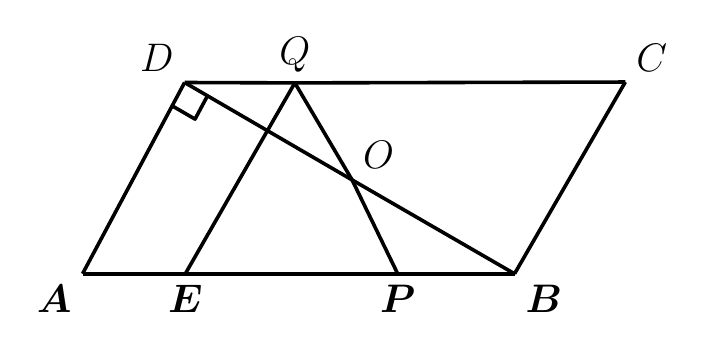
\begin{tikzpicture}[line join=round, line width=1.3pt]
\coordinate (A) at (-3.416,-1.253);
\coordinate (B) at (2.070,-1.253);
\coordinate (C) at (3.477,1.182);
\coordinate (D) at (-2.120,1.176);
\coordinate (E) at (-2.111,-1.253);
\coordinate (O) at (0.007,-0.061);
\coordinate (P) at (0.586,-1.253);
\coordinate (Q) at (-0.720,1.171);




\draw (D)--(Q)--(C);


\draw (A)--(E)--(P)--(B);

\draw (B)--(C);
\draw (A)--(D);


\draw (D)--(O)--(B);

\draw (Q)--(E);


\draw (Q)--(O)--(P);


\draw pic[draw,angle radius=0.336cm] {right angle=A--D--B};


\node[below left, font=\fontsize{13.5}{16.2}\selectfont] at (A) {$\boldsymbol{A}$};
\node[below right, font=\fontsize{13.5}{16.2}\selectfont] at (B) {$\boldsymbol{B}$};
\node[above right, font=\fontsize{13.5}{16.2}\selectfont] at (C) {$C$};
\node[above left, font=\fontsize{13.5}{16.2}\selectfont] at (D) {$D$};
\node[above, font=\fontsize{13.5}{16.2}\selectfont] at (Q) {$Q$};
\node[above right, font=\fontsize{13.5}{16.2}\selectfont] at (O) {$O$};
\node[below, font=\fontsize{13.5}{16.2}\selectfont] at (E) {$\boldsymbol{E}$};
\node[below, font=\fontsize{13.5}{16.2}\selectfont] at (P) {$\boldsymbol{P}$};
\end{tikzpicture}
\end{document}